\section{Geschichte}
\begin{frame}{Geschichte}%
  \begin{columns}[c, onlytextwidth]%
    \column{0.15\textwidth}%
      \centering
      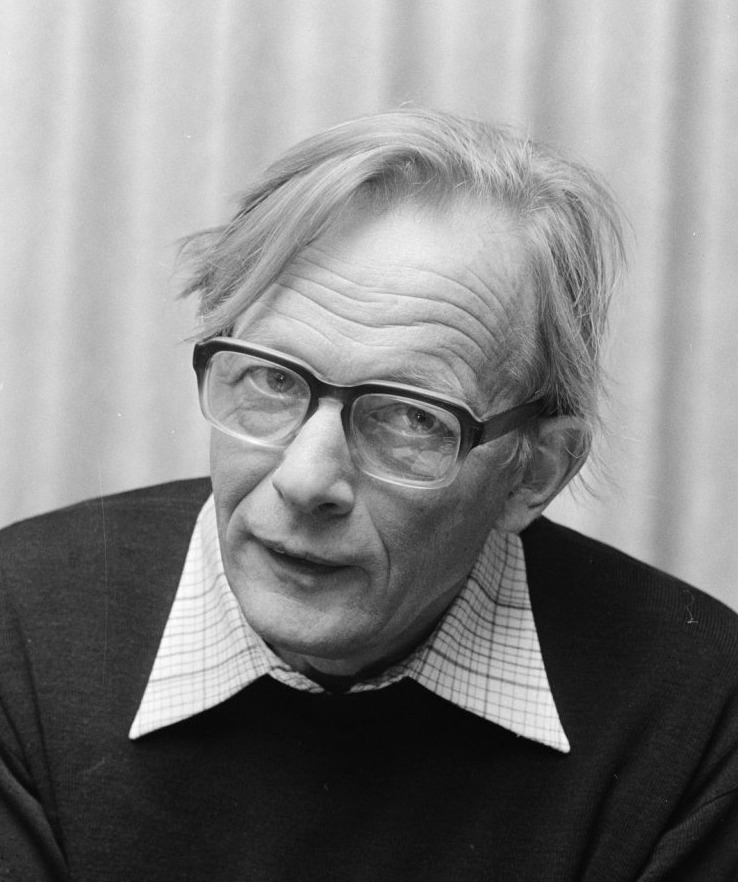
\includegraphics[width=\linewidth]{./images/Hendrik_vanDeHulst.jpg}
      \newline H. v.\,d. Hulst
    \column{0.8\textwidth}%
      \begin{description}[Hendrik van de Hulst]
        \item[Hendrik van de Hulst] Holländischer Astronom \& Mathematiker
        \item[1944] Vorhersage der \SI{21}{\centi\meter}-Linie
        \item[später] Mitarbeit bei der Kartographie der Milchstraße
      \end{description}
  \end{columns}%
  \vfill
  \begin{columns}[c, onlytextwidth]%
    \column{0.15\textwidth}%
      \centering
      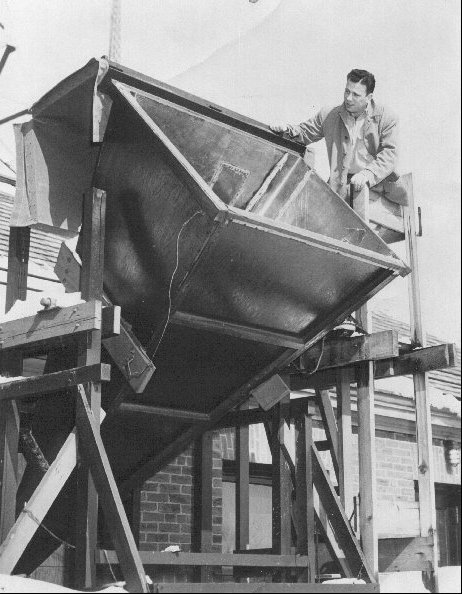
\includegraphics[width=\linewidth]{./images/ewenhorn.jpg}%
      \newline H.~Ewen
    \column{0.65\textwidth}%
      \begin{description}[1951]
        \item[1951] Entdeckung durch Edward Purcell \& Harold Ewen\\
                    an der Harvard University
      \end{description}
    \column{0.15\textwidth}%
      \centering
      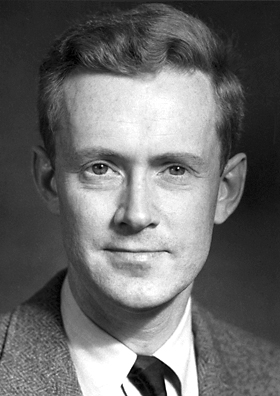
\includegraphics[width=\linewidth]{./images/Edward_Mills_Purcell.jpg}%
      \newline E.~Purcell
  \end{columns}%
\end{frame}

\begin{frame}{Die \SI{21}{\centi\meter}-Linie – Vermessung der Milchstraße}%
  \begin{columns}[c, onlytextwidth]
    \begin{column}{0.47\textwidth}%
      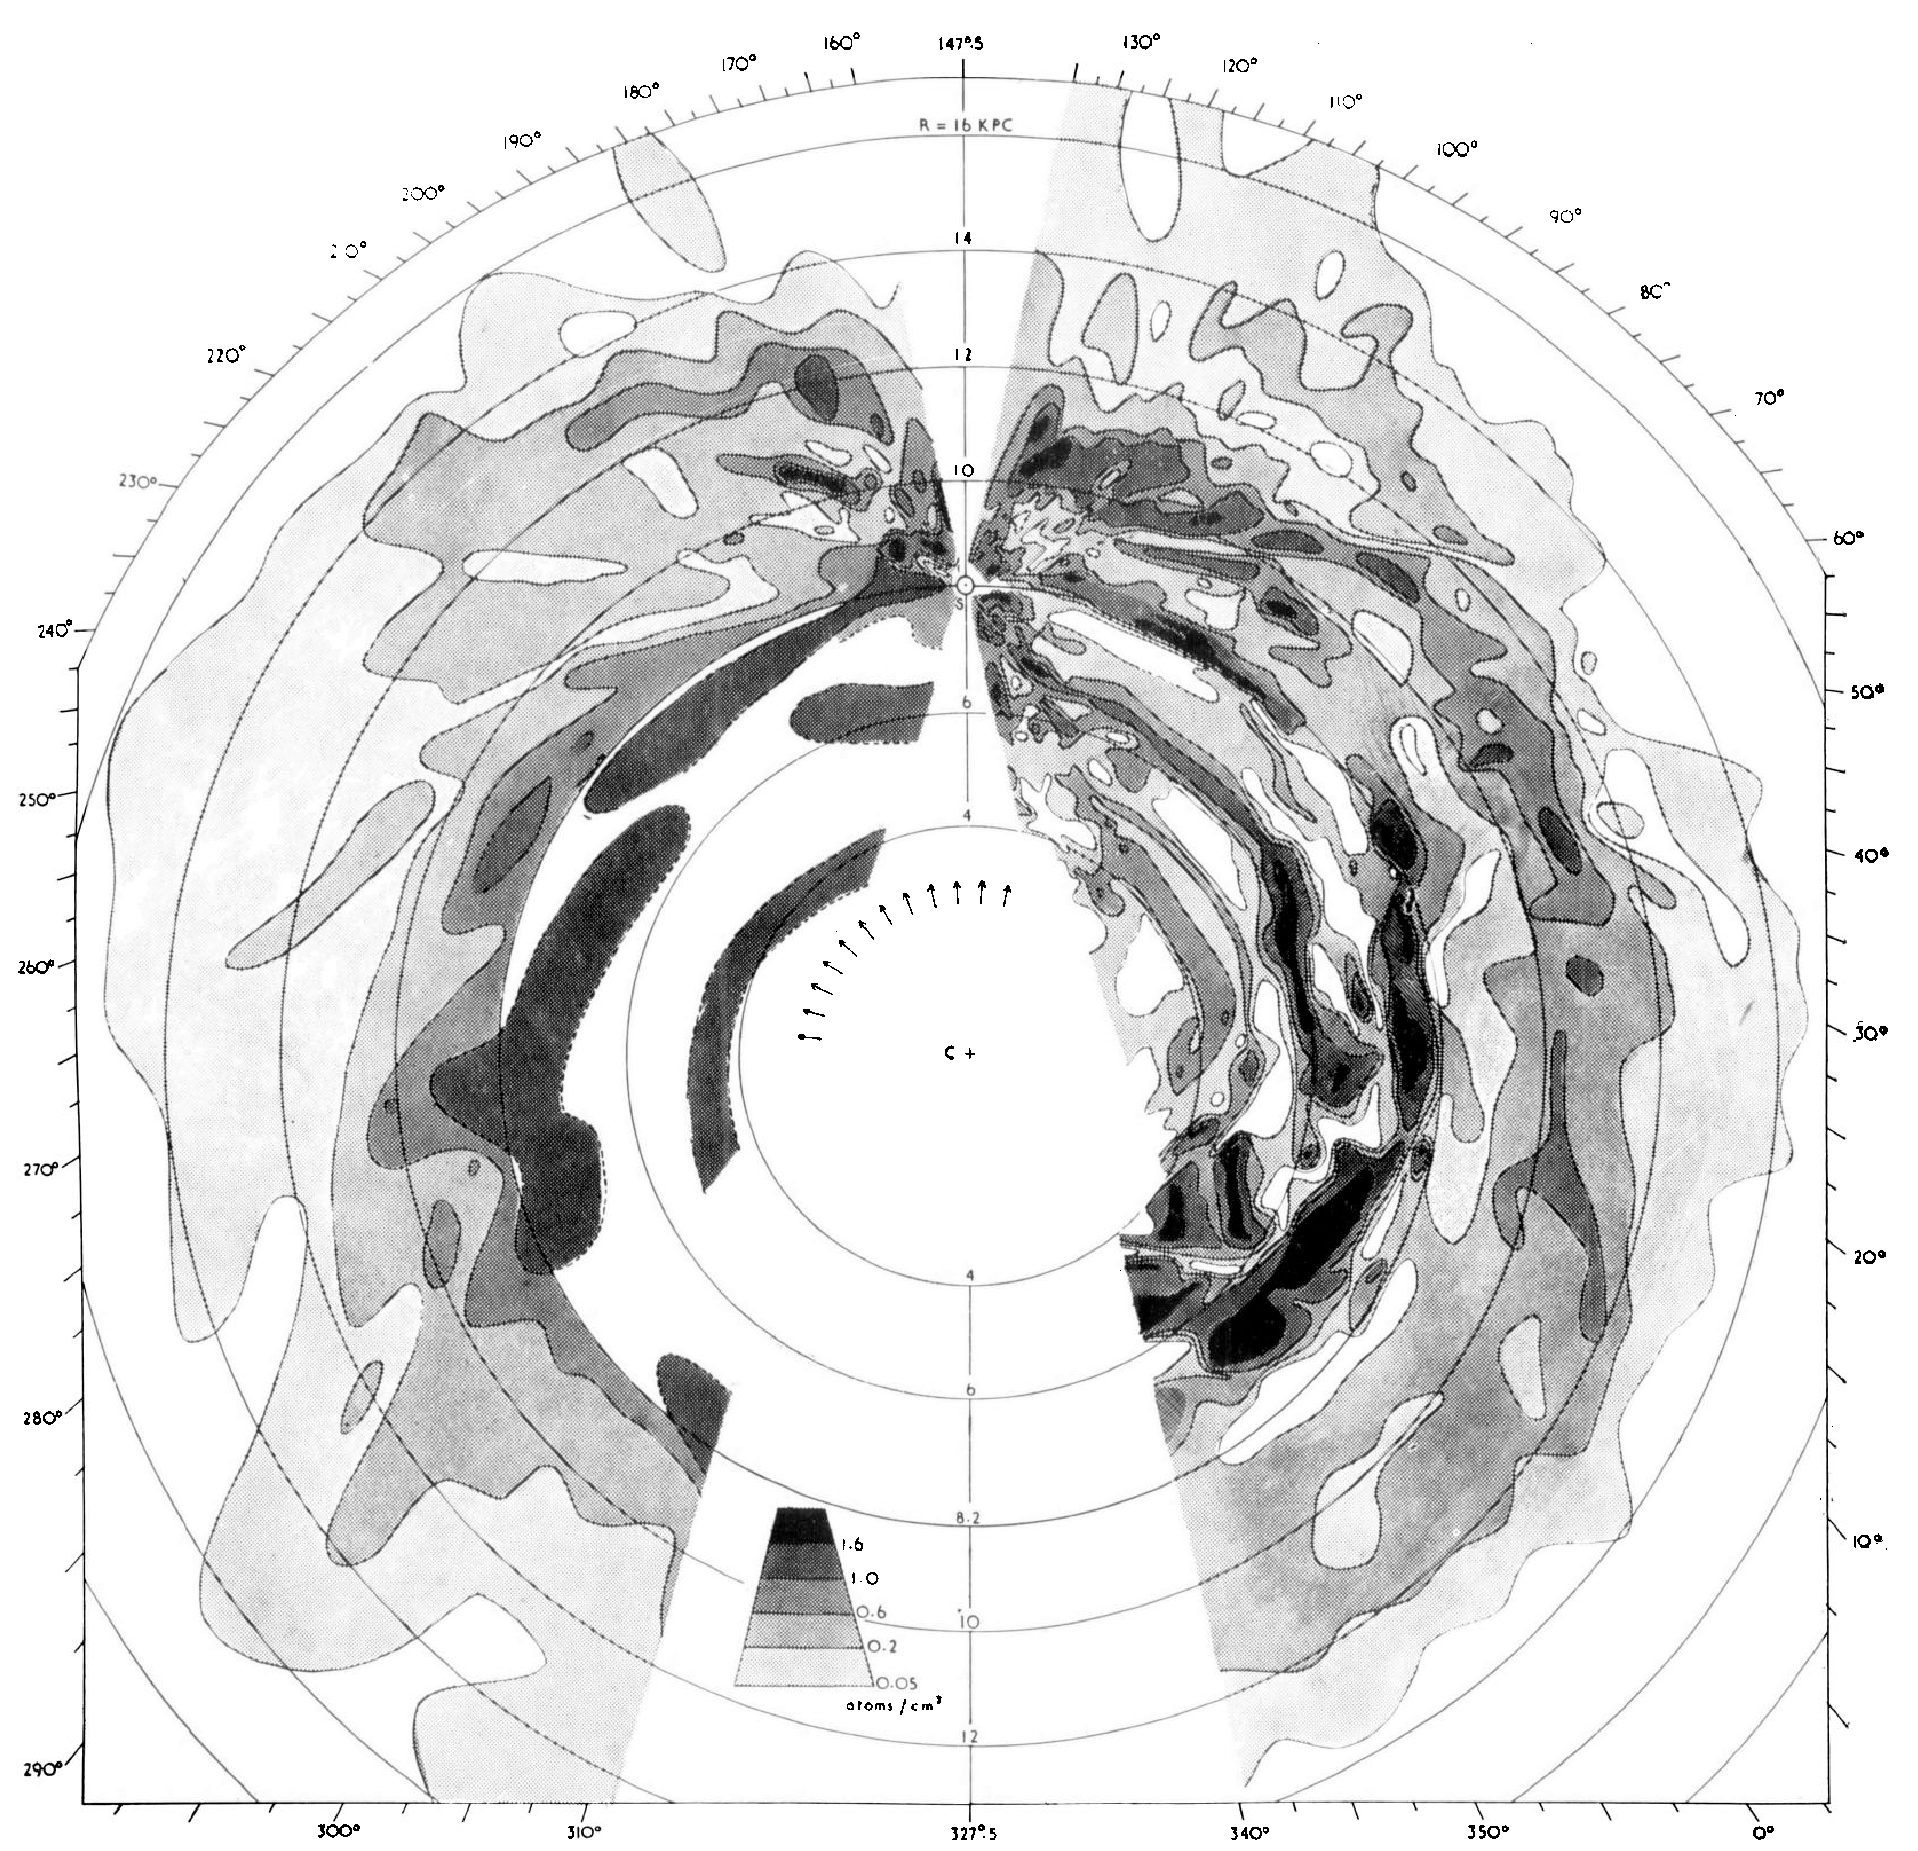
\includegraphics[width=\textwidth, angle=180]{./images/original_map.png}%
    \end{column}%
    \begin{column}{0.47\textwidth}%
      \begin{description}[Messung]
        \item[1958] Veröffentlichung der ersten \enquote{Karte} der Milchstraße
        \item[Autoren] J. H. Oort, F. J. Kerr und G. Westerhout
        \item[Messung] \SI{7.5}{\meter}-Teleskop (Leiden) \&  \SI{11}{\meter}-Teleskop (Sidney)
      \end{description}

      \begin{center}
      \parbox{0.85\linewidth}{\enquote{The \SI{21}{\centi\meter} oberservations brought about a revolution in the study of galactic structure}}
      \end{center}
    \end{column}%
  \end{columns}
\end{frame}
